\section{Risikoabsch�tzung}

\subsection{Risiko - Eintrittswahrscheinlichkeit - Schadenpotenzial}

\begin{itemize}
\item Komplexit�t: Die Schnittstelle zu Lotus Notes kann schwierig zu realisieren sein.
\item Termin: Das Projekt wird nicht zum vereinbarten Termin abgeschlossen.
\item Qualit�t: Die vereinbarten Anforderungen werden nicht erf�llt.
\item Budget: Das Projekt wird teurer als geplant.
\item �nderungen: Die Anforderungen werden nachtr�glich ge�ndert.
\end{itemize}

\begin{table}
\caption{Risiko - Eintrittswahrscheinlichkeit - Schadenpotenzial}
\begin{tabular}[h]{|p{3cm}|p{7cm}|p{4cm}|}
\hline
\textsc{Risiko} & \textsc{Eintrittswahrscheinlichkeit} & \textsc{Schadenpotenzial}\\
\hline
Komplexit�t & 0,5 & 0,5\\
\hline
Termin & 0,25 & 0,25\\
\hline
Qualit�t & 0,2 & 0,35\\
\hline
Budget & 0,05 & 0,5\\
\hline
�nderungen & 0,1 & 0,1\\
\hline
\end{tabular}
\end{table}

\begin{figure}
\begin{center}
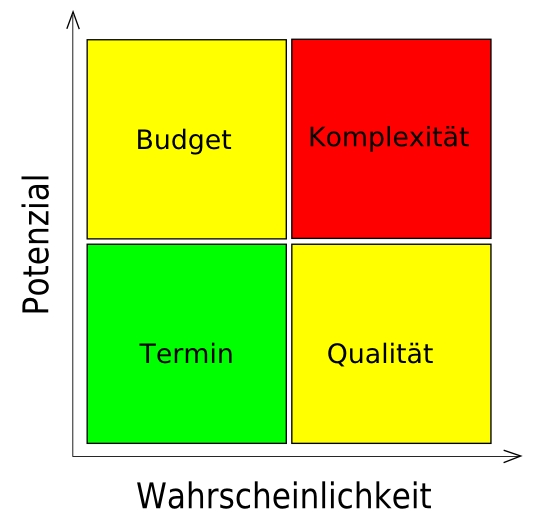
\includegraphics[width=0.8\textwidth]{abbildungen/Wahrscheinlichkeit-Potenzial.jpg}
\caption{Risiko - Eintrittswahrscheinlichkeit - Schadenpotenzial}
\end{center}
\end{figure}

\subsection{Risikomatrix}
\subsection{Vorbeugema�nahmen}
\subsection{Korrekturma�nahmen}